% Options for packages loaded elsewhere
\PassOptionsToPackage{unicode}{hyperref}
\PassOptionsToPackage{hyphens}{url}
\PassOptionsToPackage{dvipsnames,svgnames*,x11names*}{xcolor}
%
\documentclass[
]{article}
\usepackage[]{Roboto}
\usepackage{amssymb,amsmath}
\usepackage{ifxetex,ifluatex}
\ifnum 0\ifxetex 1\fi\ifluatex 1\fi=0 % if pdftex
  \usepackage[T1]{fontenc}
  \usepackage[utf8]{inputenc}
  \usepackage{textcomp} % provide euro and other symbols
\else % if luatex or xetex
  \usepackage{unicode-math}
  \defaultfontfeatures{Scale=MatchLowercase}
  \defaultfontfeatures[\rmfamily]{Ligatures=TeX,Scale=1}
\fi
% Use upquote if available, for straight quotes in verbatim environments
\IfFileExists{upquote.sty}{\usepackage{upquote}}{}
\IfFileExists{microtype.sty}{% use microtype if available
  \usepackage[]{microtype}
  \UseMicrotypeSet[protrusion]{basicmath} % disable protrusion for tt fonts
}{}
\makeatletter
\@ifundefined{KOMAClassName}{% if non-KOMA class
  \IfFileExists{parskip.sty}{%
    \usepackage{parskip}
  }{% else
    \setlength{\parindent}{0pt}
    \setlength{\parskip}{6pt plus 2pt minus 1pt}}
}{% if KOMA class
  \KOMAoptions{parskip=half}}
\makeatother
\usepackage{xcolor}
\IfFileExists{xurl.sty}{\usepackage{xurl}}{} % add URL line breaks if available
\IfFileExists{bookmark.sty}{\usepackage{bookmark}}{\usepackage{hyperref}}
\hypersetup{
  pdftitle={RMarkdown Template},
  pdfauthor={Nina West; Trixie Mattel; Chi Chi Devayne},
  colorlinks=true,
  linkcolor=Maroon,
  filecolor=Maroon,
  citecolor=Blue,
  urlcolor=blue,
  pdfcreator={LaTeX via pandoc}}
\urlstyle{same} % disable monospaced font for URLs
\usepackage[margin=1in]{geometry}
\usepackage{color}
\usepackage{fancyvrb}
\newcommand{\VerbBar}{|}
\newcommand{\VERB}{\Verb[commandchars=\\\{\}]}
\DefineVerbatimEnvironment{Highlighting}{Verbatim}{commandchars=\\\{\}}
% Add ',fontsize=\small' for more characters per line
\usepackage{framed}
\definecolor{shadecolor}{RGB}{248,248,248}
\newenvironment{Shaded}{\begin{snugshade}}{\end{snugshade}}
\newcommand{\AlertTok}[1]{\textcolor[rgb]{0.94,0.16,0.16}{#1}}
\newcommand{\AnnotationTok}[1]{\textcolor[rgb]{0.56,0.35,0.01}{\textbf{\textit{#1}}}}
\newcommand{\AttributeTok}[1]{\textcolor[rgb]{0.77,0.63,0.00}{#1}}
\newcommand{\BaseNTok}[1]{\textcolor[rgb]{0.00,0.00,0.81}{#1}}
\newcommand{\BuiltInTok}[1]{#1}
\newcommand{\CharTok}[1]{\textcolor[rgb]{0.31,0.60,0.02}{#1}}
\newcommand{\CommentTok}[1]{\textcolor[rgb]{0.56,0.35,0.01}{\textit{#1}}}
\newcommand{\CommentVarTok}[1]{\textcolor[rgb]{0.56,0.35,0.01}{\textbf{\textit{#1}}}}
\newcommand{\ConstantTok}[1]{\textcolor[rgb]{0.00,0.00,0.00}{#1}}
\newcommand{\ControlFlowTok}[1]{\textcolor[rgb]{0.13,0.29,0.53}{\textbf{#1}}}
\newcommand{\DataTypeTok}[1]{\textcolor[rgb]{0.13,0.29,0.53}{#1}}
\newcommand{\DecValTok}[1]{\textcolor[rgb]{0.00,0.00,0.81}{#1}}
\newcommand{\DocumentationTok}[1]{\textcolor[rgb]{0.56,0.35,0.01}{\textbf{\textit{#1}}}}
\newcommand{\ErrorTok}[1]{\textcolor[rgb]{0.64,0.00,0.00}{\textbf{#1}}}
\newcommand{\ExtensionTok}[1]{#1}
\newcommand{\FloatTok}[1]{\textcolor[rgb]{0.00,0.00,0.81}{#1}}
\newcommand{\FunctionTok}[1]{\textcolor[rgb]{0.00,0.00,0.00}{#1}}
\newcommand{\ImportTok}[1]{#1}
\newcommand{\InformationTok}[1]{\textcolor[rgb]{0.56,0.35,0.01}{\textbf{\textit{#1}}}}
\newcommand{\KeywordTok}[1]{\textcolor[rgb]{0.13,0.29,0.53}{\textbf{#1}}}
\newcommand{\NormalTok}[1]{#1}
\newcommand{\OperatorTok}[1]{\textcolor[rgb]{0.81,0.36,0.00}{\textbf{#1}}}
\newcommand{\OtherTok}[1]{\textcolor[rgb]{0.56,0.35,0.01}{#1}}
\newcommand{\PreprocessorTok}[1]{\textcolor[rgb]{0.56,0.35,0.01}{\textit{#1}}}
\newcommand{\RegionMarkerTok}[1]{#1}
\newcommand{\SpecialCharTok}[1]{\textcolor[rgb]{0.00,0.00,0.00}{#1}}
\newcommand{\SpecialStringTok}[1]{\textcolor[rgb]{0.31,0.60,0.02}{#1}}
\newcommand{\StringTok}[1]{\textcolor[rgb]{0.31,0.60,0.02}{#1}}
\newcommand{\VariableTok}[1]{\textcolor[rgb]{0.00,0.00,0.00}{#1}}
\newcommand{\VerbatimStringTok}[1]{\textcolor[rgb]{0.31,0.60,0.02}{#1}}
\newcommand{\WarningTok}[1]{\textcolor[rgb]{0.56,0.35,0.01}{\textbf{\textit{#1}}}}
\usepackage{graphicx}
\makeatletter
\def\maxwidth{\ifdim\Gin@nat@width>\linewidth\linewidth\else\Gin@nat@width\fi}
\def\maxheight{\ifdim\Gin@nat@height>\textheight\textheight\else\Gin@nat@height\fi}
\makeatother
% Scale images if necessary, so that they will not overflow the page
% margins by default, and it is still possible to overwrite the defaults
% using explicit options in \includegraphics[width, height, ...]{}
\setkeys{Gin}{width=\maxwidth,height=\maxheight,keepaspectratio}
% Set default figure placement to htbp
\makeatletter
\def\fps@figure{htbp}
\makeatother
\setlength{\emergencystretch}{3em} % prevent overfull lines
\providecommand{\tightlist}{%
  \setlength{\itemsep}{0pt}\setlength{\parskip}{0pt}}
\setcounter{secnumdepth}{-\maxdimen} % remove section numbering
\usepackage{float}

\title{RMarkdown Template}
\author{Nina West \and Trixie Mattel \and Chi Chi Devayne}
\date{August 16th, 2021}

\begin{document}
\maketitle

\hypertarget{rmarkdown-is-awesome}{%
\section{RMarkdown is awesome}\label{rmarkdown-is-awesome}}

It make take a bit more time, but the flexibility that Rmarkdown gives
you (and the aesthetics \textbf{*chef's kiss*}) is unbeatable. This file
is meant to act as a template and it includes some basic comments (both
here and in the accompanying .css file, if you want to go to the HTML
dark side), so it can be easily customized.

Don't despair! You might start like this:

\begin{figure}
\centering

\includegraphics[width=3in,height=\textheight]{./Rmarkdown/images/knits2.png}
\caption{Dog is knitting angrily}
\end{figure}

But you will end up like this\footnote{Note how we are changing the size
  of these figures (you can use different measures!)}:

\begin{figure}
\centering

\includegraphics[width=0.4\textwidth,height=\textheight]{./Rmarkdown/images/cool_beans.jpeg}
\caption{Cool beans!}
\end{figure}

You can see the knitted version (PDF) of this file
\href{https://www.magdalenabennett.com/files/Rmarkdown_template.pdf}{here}

\hypertarget{lets-see-some-examples}{%
\section{Let's see some examples}\label{lets-see-some-examples}}

\hypertarget{how-does-work-in-rmarkdown}{%
\subsection{\texorpdfstring{How does \LaTeX work in
RMarkdown?}{How does work in RMarkdown?}}\label{how-does-work-in-rmarkdown}}

Well, it works pretty much the same as \LaTeX on its own (if you are
familiar with it). Include inline equations like:
\(y_i = \beta_0 + \beta_1\cdot x_i + \varepsilon_i\), or equations on
their own line:

\[y_i = \beta_0 + \beta_1 x_{i1} + \beta_2 x_{i2} + \beta_3 x_{i3} + \beta_4 x_{i4} + ... + \varepsilon_{i}\]

In this case \texttt{\textbackslash{}beta} basically compiles as
\(\beta\), and the underscore creates a subindex, just like this:
\(\beta_0\). How can we do a superscript? Easy!
\texttt{\textbackslash{}theta\^{}\{ATE\}}, which knits as
\(\theta^{ATE}\) (Note: Why do we use curly braces for this superscript?
Try out what happens when you don't use those braces\ldots)

The previous equation looks good, but sometimes they are too long to be
included in one line. What to do? use
\texttt{\textbackslash{}\textbackslash{}} to break lines within an
equation. At the same time, you might want lines to be aligned at the
equal sign. Here is how you do that:

\[\begin{aligned}
y_i =& \beta_0 + \beta_1 x_{i1} + \beta_2 x_{i2} + \beta_3 x_{i3} +\\
    &\beta_4 x_{i4} + ... + \varepsilon_{i}
\end{aligned}\]

(Note: Notice that the \texttt{\&} sign denotes how the lines should be
aligned).

\begin{center}\rule{0.5\linewidth}{0.5pt}\end{center}

\hypertarget{lets-code}{%
\subsection{Let's code}\label{lets-code}}

We can write some simple code, if we want to show it (\emph{Tip: Include
\texttt{message=FALSE} and \texttt{warning=FALSE} so you don't get that
extra stuff when you run the code}):

\begin{Shaded}
\begin{Highlighting}[]
\KeywordTok{data}\NormalTok{(cars)}

\KeywordTok{lm}\NormalTok{(speed }\OperatorTok{\textasciitilde{}}\StringTok{ }\NormalTok{dist, }\DataTypeTok{data =}\NormalTok{ cars)}
\end{Highlighting}
\end{Shaded}

\begin{verbatim}
## 
## Call:
## lm(formula = speed ~ dist, data = cars)
## 
## Coefficients:
## (Intercept)         dist  
##      8.2839       0.1656
\end{verbatim}

Meh, but that output looks ugly. Can we make it prettier? Let's try
\texttt{stargazer} (you will need to include the
\texttt{results=\textquotesingle{}asis\textquotesingle{}} argument).

\begin{table}[H] \centering 
  \caption{Regression of Speed on Distance} 
  \label{} 
\begin{tabular}{@{\extracolsep{5pt}}lc} 
\\[-1.8ex]\hline 
\hline \\[-1.8ex] 
 & \multicolumn{1}{c}{Dependent Variable: Speed} \\ 
\cline{2-2} 
\\[-1.8ex] &  \\ 
 & Model 1 \\ 
\hline \\[-1.8ex] 
 dist & 0.166$^{***}$ \\ 
  & (0.017) \\ 
  & \\ 
 Constant & 8.284$^{***}$ \\ 
  & (0.874) \\ 
  & \\ 
\hline \\[-1.8ex] 
Observations & 50 \\ 
R$^{2}$ & 0.651 \\ 
Adjusted R$^{2}$ & 0.644 \\ 
Residual Std. Error & 3.156 (df = 48) \\ 
F Statistic & 89.567$^{***}$ (df = 1; 48) \\ 
\hline 
\hline \\[-1.8ex] 
\textit{Note:}  & \multicolumn{1}{r}{$^{*}$p$<$0.1; $^{**}$p$<$0.05; $^{***}$p$<$0.01} \\ 
\end{tabular} 
\end{table}

You can also compare more than one model:

\begin{table}[H] \centering 
  \caption{Two Regressions of Speed on Distance} 
  \label{} 
\begin{tabular}{@{\extracolsep{5pt}}lcc} 
\\[-1.8ex]\hline 
\hline \\[-1.8ex] 
 & \multicolumn{2}{c}{Dependent Variable: Speed} \\ 
\cline{2-3} 
\\[-1.8ex] & \multicolumn{2}{c}{} \\ 
 & Model 1 & Model 2 \\ 
\\[-1.8ex] & (1) & (2)\\ 
\hline \\[-1.8ex] 
 distance & 0.166$^{***}$ & 0.327$^{***}$ \\ 
  & (0.017) & (0.055) \\ 
  & & \\ 
 distance$^2$ &  & $-$0.002$^{***}$ \\ 
  &  & (0.0005) \\ 
  & & \\ 
 Constant & 8.284$^{***}$ & 5.144$^{***}$ \\ 
  & (0.874) & (1.295) \\ 
  & & \\ 
\hline \\[-1.8ex] 
Observations & 50 & 50 \\ 
R$^{2}$ & 0.651 & 0.710 \\ 
Adjusted R$^{2}$ & 0.644 & 0.698 \\ 
Residual Std. Error & 3.156 (df = 48) & 2.907 (df = 47) \\ 
F Statistic & 89.567$^{***}$ (df = 1; 48) & 57.573$^{***}$ (df = 2; 47) \\ 
\hline 
\hline \\[-1.8ex] 
\textit{Note:}  & \multicolumn{2}{r}{$^{*}$p$<$0.1; $^{**}$p$<$0.05; $^{***}$p$<$0.01} \\ 
\end{tabular} 
\end{table}

\begin{center}\rule{0.5\linewidth}{0.5pt}\end{center}

\hypertarget{lets-plot}{%
\section{Let's plot}\label{lets-plot}}

Finally, let's briefly look into plots. Play around with this syntax to
customize it however you want!

\begin{figure}[H]

{\centering 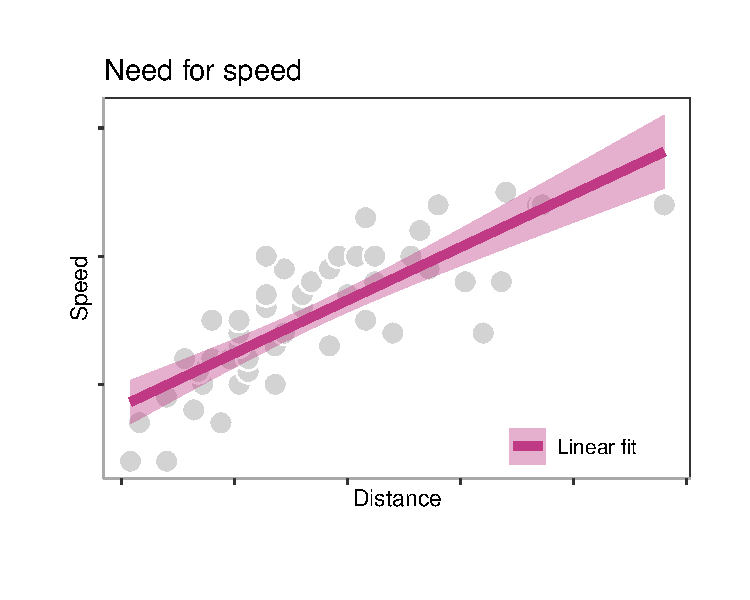
\includegraphics[width=0.7\linewidth]{Rmarkdown_template_files/figure-latex/speed1-1} 

}

\caption{This is my first plot}\label{fig:speed1}
\end{figure}

\ldots{} and for Andrew Baker's sake, we can also rotate the y-axis
label (remember to rename your code chunk!)

\begin{figure}[H]

{\centering 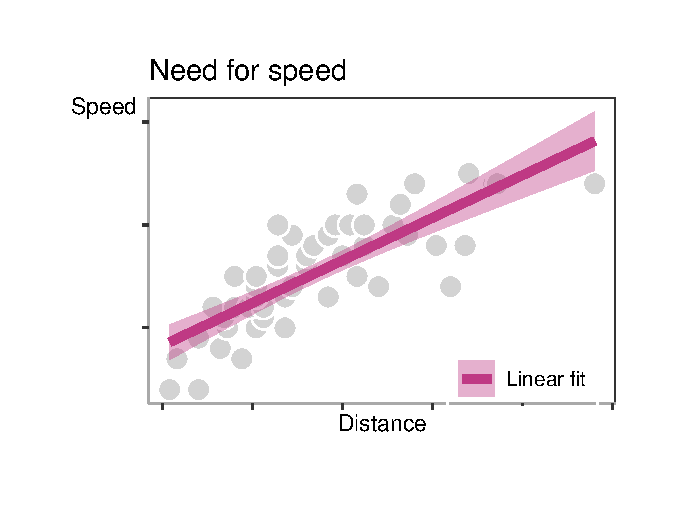
\includegraphics{Rmarkdown_template_files/figure-latex/speed2-1} 

}

\caption{This is my second plot}\label{fig:speed2}
\end{figure}

\begin{center}\rule{0.5\linewidth}{0.5pt}\end{center}

\hypertarget{come-to-the-dark-html-side}{%
\section{Come to the dark {[}HTML{]}
side\ldots{}}\label{come-to-the-dark-html-side}}

If you want to see how this would look as HTML, just change your YAML
(i.e.~the header of this document, between --- and ---) for the
following:

\begin{verbatim}
---
title: "RMarkdown Template" # You can put the title of your document here
author: 
  - Nina West  # You can include names here
  - Trixie Mattel
  - Chi Chi Devayne
date: "August 16th, 2021"
output: 
  html_document:
    css: style.css 
    toc: no
---
\end{verbatim}

I've included a separate
\href{https://raw.githubusercontent.com/maibennett/website_github/master/exampleSite/content/files/Rmarkdown_template.Rmd}{R
markdown file} with this\footnote{Note that if you want to use CSS
  styles, you'll need to include the
  \href{https://raw.githubusercontent.com/maibennett/website_github/master/exampleSite/content/files/style.css}{style.css}
  file in the same directory as your .Rmd file}, that you can knit and
see how the HTML file looks. I've also uploaded it
\href{https://www.magdalenabennett.com/files/Rmarkdown_template.html}{here}
just for fun.

If you want to share your HTML files, a super quick way is
\href{https://twitter.com/grant_mcdermott}{Grant McDermottt's}
suggestion using Github:

\begin{figure}
\centering
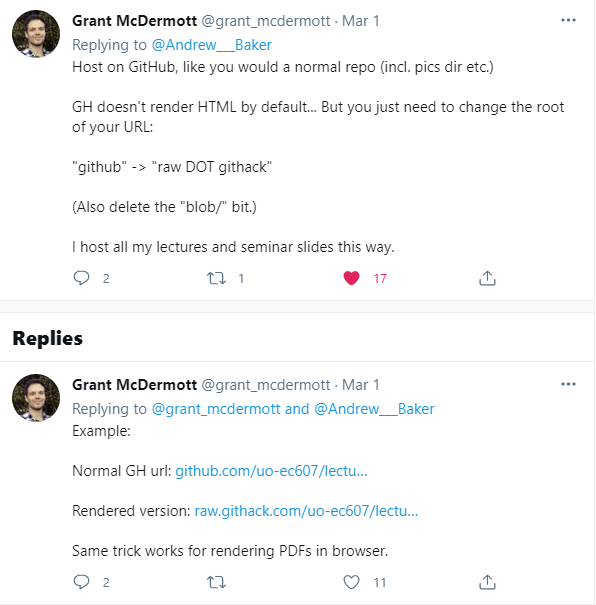
\includegraphics[width=0.5\textwidth,height=\textheight]{./Rmarkdown/images/host_html.png}
\caption{Twitter is great}
\end{figure}

\end{document}
